\documentclass[11pt]{article}

\usepackage[utf8]{inputenc}
\usepackage[spanish]{babel}
\usepackage[margin=2.5cm]{geometry}
\usepackage{graphicx}
\usepackage{hyperref}
\usepackage{xcolor}
\usepackage{listings}
\usepackage{booktabs}
\usepackage{caption}

\graphicspath{{images/}}

\hypersetup{
    colorlinks=true,
    linkcolor=blue,
    urlcolor=blue,
    citecolor=blue,
    pdftitle={Spacecraft Engines Data Pipeline},
    pdfauthor={Stan Mora, Tais Rodriguez}
}

\lstset{
    basicstyle=\ttfamily\small,
    breaklines=true,
    frame=single,
    backgroundcolor=\color{gray!10},
    columns=fullflexible,
}

\title{\textbf{Spacecraft Engines Data Pipeline} \\
\large Proyecto Final -- Ingeniería de Datos \\
\large Pipeline de datos batch y streaming en tiempo real sobre motores de cohetes espaciales, desplegado en AWS real}
\author{Stan Mora \and Tais Rodriguez}
\date{\today}

\begin{document}

\maketitle
\tableofcontents
\newpage

% ============================================================
\section{Introducción y objetivo}
% ============================================================

Este proyecto implementa un pipeline de datos completo sobre motores de cohetes espaciales, cubriendo los dos tipos de flujo requeridos por el curso: procesamiento \textbf{batch} (histórico de lanzamientos) y procesamiento \textbf{streaming en tiempo real} (telemetría simulada de motores). Ambos flujos están desplegados sobre servicios reales de AWS -- no simulaciones locales únicamente -- e incluyen ingesta desde múltiples fuentes, transformación, almacenamiento, un modelo de machine learning, un detector de anomalías en tiempo real, y un dashboard interactivo que consolida ambos flujos en una sola pantalla.

El objetivo es demostrar, de punta a punta, el ciclo completo de un pipeline moderno de datos: ingesta $\rightarrow$ almacenamiento $\rightarrow$ transformación $\rightarrow$ análisis/modelado $\rightarrow$ visualización, con infraestructura real (no simulada) donde corresponde, y con desarrollo local reproducible antes de tocar la nube.

% ============================================================
\section{Fuentes de datos}
% ============================================================

El proyecto ingiere datos de \textbf{dos fuentes independientes}, cumpliendo el requisito de ingesta multi-fuente:

\begin{enumerate}
    \item \textbf{Launch Library 2 API} (\texttt{ll.thespacedevs.com}) -- API pública, gratuita y sin necesidad de clave de autenticación, que provee el histórico real de lanzamientos espaciales de múltiples agencias: SpaceX, NASA, Roscosmos, ESA, Rocket Lab y Blue Origin. Se consulta una vez por familia de cohete conocida.

    \item \textbf{Tabla estática de especificaciones de motores} (\texttt{src/batch/engine\_specs.py}) -- un archivo Python con especificaciones reales y públicamente documentadas (empuje, impulso específico, tipo de propelente) de 10 motores de cohetes: Merlin~1D, Rocketdyne~F-1, RS-25, RD-108A, RD-180, RS-68A, Vulcain~2, Rutherford y BE-4. No proviene de una API porque no existe ninguna fuente gratuita con ese nivel de detalle por motor -- son valores físicos reales, ampliamente citados públicamente.
\end{enumerate}

% ============================================================
\section{Arquitectura general}
% ============================================================

La Figura~\ref{fig:arch} muestra la arquitectura completa: dos flujos paralelos e independientes que convergen en un único dashboard.

\begin{figure}[h]
    \centering
    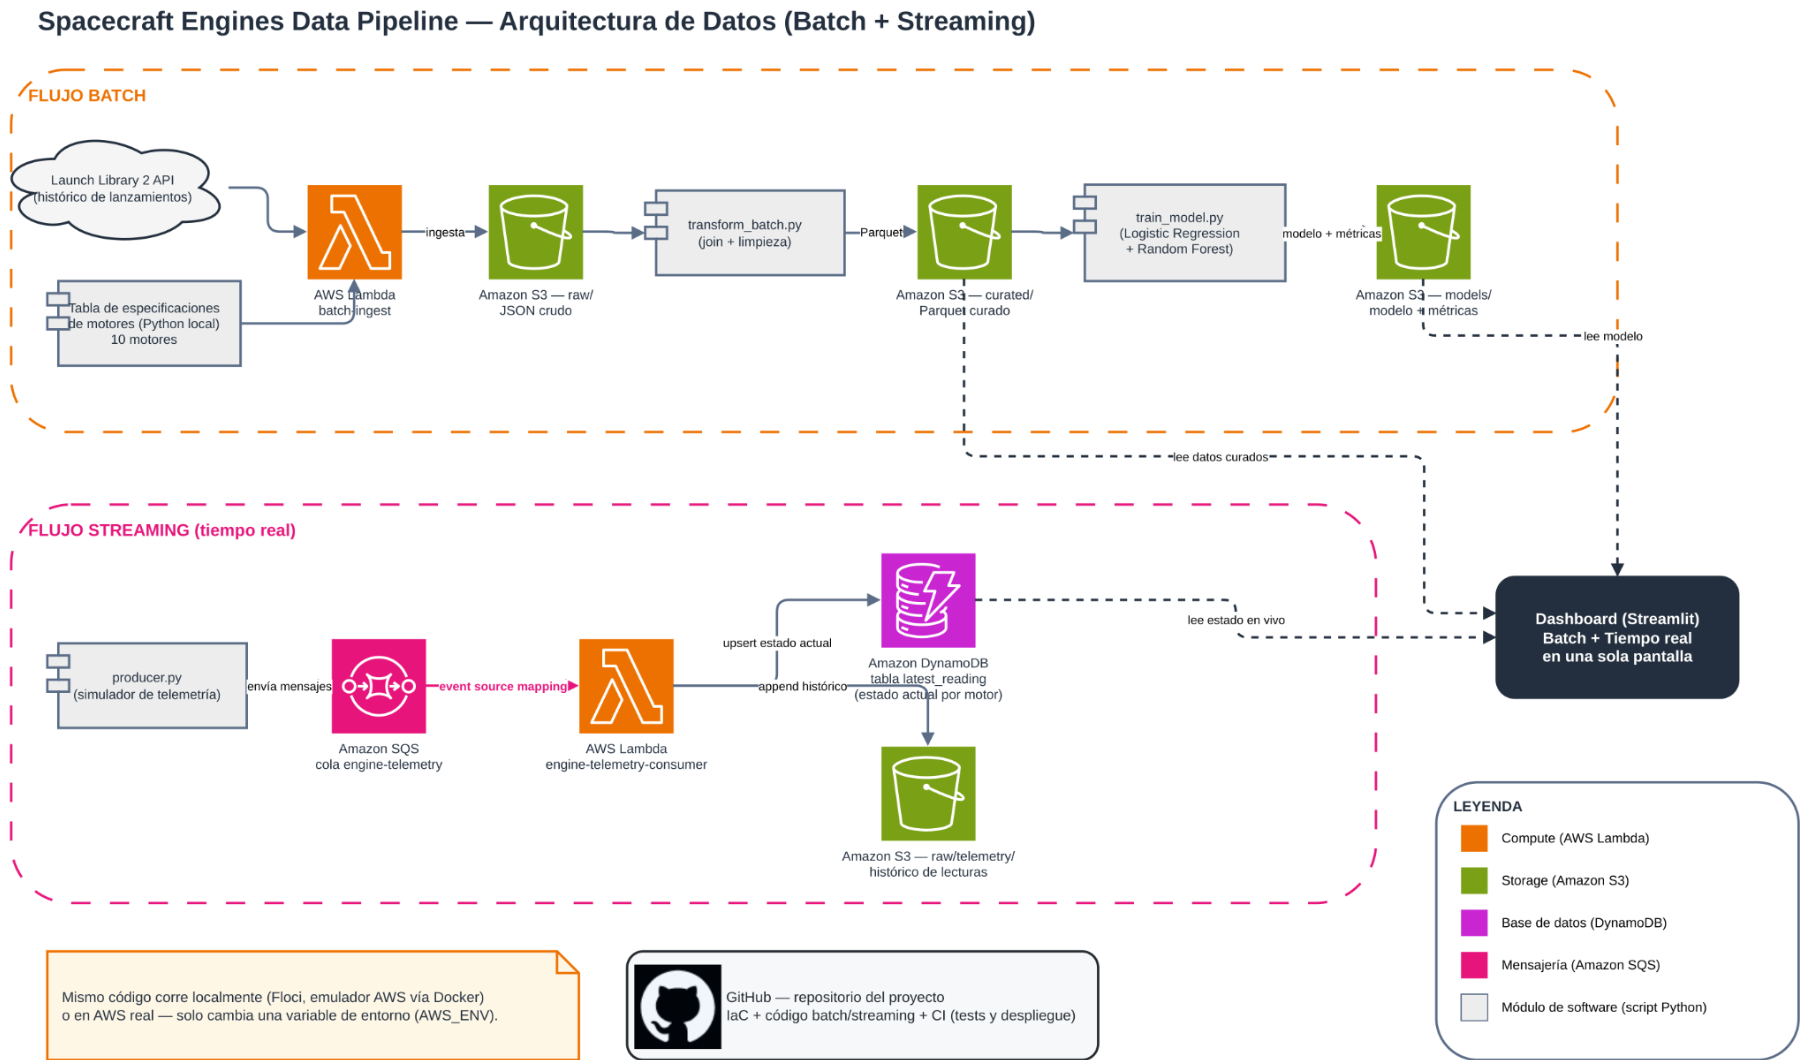
\includegraphics[width=\textwidth]{Architecture.png}
    \caption{Arquitectura general del pipeline -- flujo batch (arriba) y flujo streaming (abajo), convergiendo en el dashboard.}
    \label{fig:arch}
\end{figure}

Un aspecto de diseño importante: \textbf{el mismo código corre indistintamente en local (contra Floci, un emulador de AWS tipo LocalStack ejecutado vía Docker) o contra AWS real} -- el único cambio es una variable de entorno (\texttt{AWS\_ENV=local} vs \texttt{AWS\_ENV=aws}) en el archivo \texttt{.env}. Esto permite desarrollar y probar todo el pipeline sin costo ni riesgo antes de desplegarlo contra la cuenta real de AWS.

\newpage
% ============================================================
\section{Flujo Batch}
% ============================================================

\subsection{Ingesta}
La ingesta batch corre como una función \textbf{AWS Lambda real} (\texttt{batch-ingest}), desplegada mediante \texttt{infra/deploy\_ingest\_lambda.py}. Esta Lambda:
\begin{itemize}
    \item Consulta Launch Library~2 una vez por cada familia de cohete conocida.
    \item Escribe la tabla de especificaciones de motores y los lanzamientos crudos (JSON sin procesar) al bucket S3, bajo \texttt{raw/}.
    \item Es idempotente: si una familia ya fue ingerida, la omite en corridas posteriores en lugar de volver a consultar la API.
\end{itemize}

\subsection{Transformación}
El script \texttt{transform\_batch.py} lee los archivos JSON crudos desde S3, los combina (\textit{join}) con la tabla de especificaciones por familia de cohete, limpia inconsistencias de la fuente (por ejemplo, la búsqueda difusa de la API mezclaba resultados de familias distintas -- el caso de Atlas~V se excluye explícitamente por esta razón, documentado en el propio código), y escribe el resultado curado en formato \textbf{Parquet} a \texttt{S3 -- curated/}.

\subsection{Modelo de Machine Learning}
\texttt{train\_model.py} entrena dos modelos (Regresión Logística y Random Forest) para predecir el éxito o fallo de un lanzamiento individual, a partir de las especificaciones del motor y el año del lanzamiento. Los resultados y modelos entrenados se guardan en \texttt{S3 -- models/}.

\textbf{Resultado honesto:} la señal predictiva a nivel de lanzamiento individual es débil (ROC-AUC $\approx 0.64$), y la variable \texttt{year} domina la importancia de features (85\%) -- ya que las especificaciones del motor son constantes dentro de cada familia de cohete. Sin embargo, existe un hallazgo descriptivo más sólido: \textbf{la tasa de éxito varía genuinamente por familia de cohete} (desde 100\% en Falcon Heavy hasta 92\% en Saturn~V), lo cual se reporta con transparencia en el dashboard en lugar de sobrevender el resultado del modelo predictivo.

\newpage
% ============================================================
\section{Flujo Streaming (tiempo real)}
% ============================================================

\subsection{Simulación de telemetría}
\texttt{producer.py} simula lecturas de telemetría (empuje, presión de cámara, temperatura, vibración, flujo de combustible) para cada uno de los 10 motores. Los valores \textbf{no son aleatorios}: se derivan de física real -- por ejemplo, el flujo de combustible se calcula con la ecuación del cohete ($F = I_{sp} \cdot g_0 \cdot \dot{m}$) usando el empuje e impulso específico reales de cada motor. Ocasionalmente se inyecta una anomalía deliberada (un pico o caída en un campo), y cada inyección queda registrada como \textit{ground truth} en S3 para poder validar el detector después.

\subsection{Procesamiento en tiempo real}
Cada lectura se envía a una cola real de \textbf{Amazon SQS} (\texttt{engine-telemetry}). Esa cola dispara automáticamente -- mediante un \textit{event source mapping}, sin necesidad de invocación manual ni \textit{polling} -- una función \textbf{AWS Lambda real} (\texttt{engine-telemetry-consumer}). Esta Lambda:
\begin{itemize}
    \item Mantiene estadísticas móviles (media y varianza) por motor usando el \textbf{algoritmo de Welford}, con el estado persistido en DynamoDB entre invocaciones.
    \item Calcula un \textit{z-score} por campo y marca una lectura como anómala si supera un umbral.
    \item Escribe el estado actual (\textit{upsert}) en \textbf{DynamoDB} (\texttt{tabla latest\_reading}, un registro por motor) y archiva el lote crudo completo en \textbf{S3} (\texttt{raw/telemetry/}), esta última de forma histórica y sin sobrescritura.
\end{itemize}

\subsection{Validación del detector de anomalías}
\texttt{validate\_anomaly\_detector.py} compara las anomalías detectadas por la Lambda contra el \textit{ground truth} inyectado por el propio simulador, obteniendo \textbf{95\% de recall y 76\% de precisión} -- una validación real y medible, no una suposición de que el detector funciona correctamente.

\newpage
% ============================================================
\section{Entorno de desarrollo local (Floci)}
% ============================================================

Todo el desarrollo y las pruebas se realizaron primero contra \textbf{Floci}, un emulador de AWS local (tipo LocalStack) ejecutado vía Docker Compose, sin necesidad de credenciales reales ni costo. Esto permitió iterar rápidamente y validar toda la lógica antes de desplegar contra la cuenta real de AWS.

\begin{figure}[h]
    \centering
    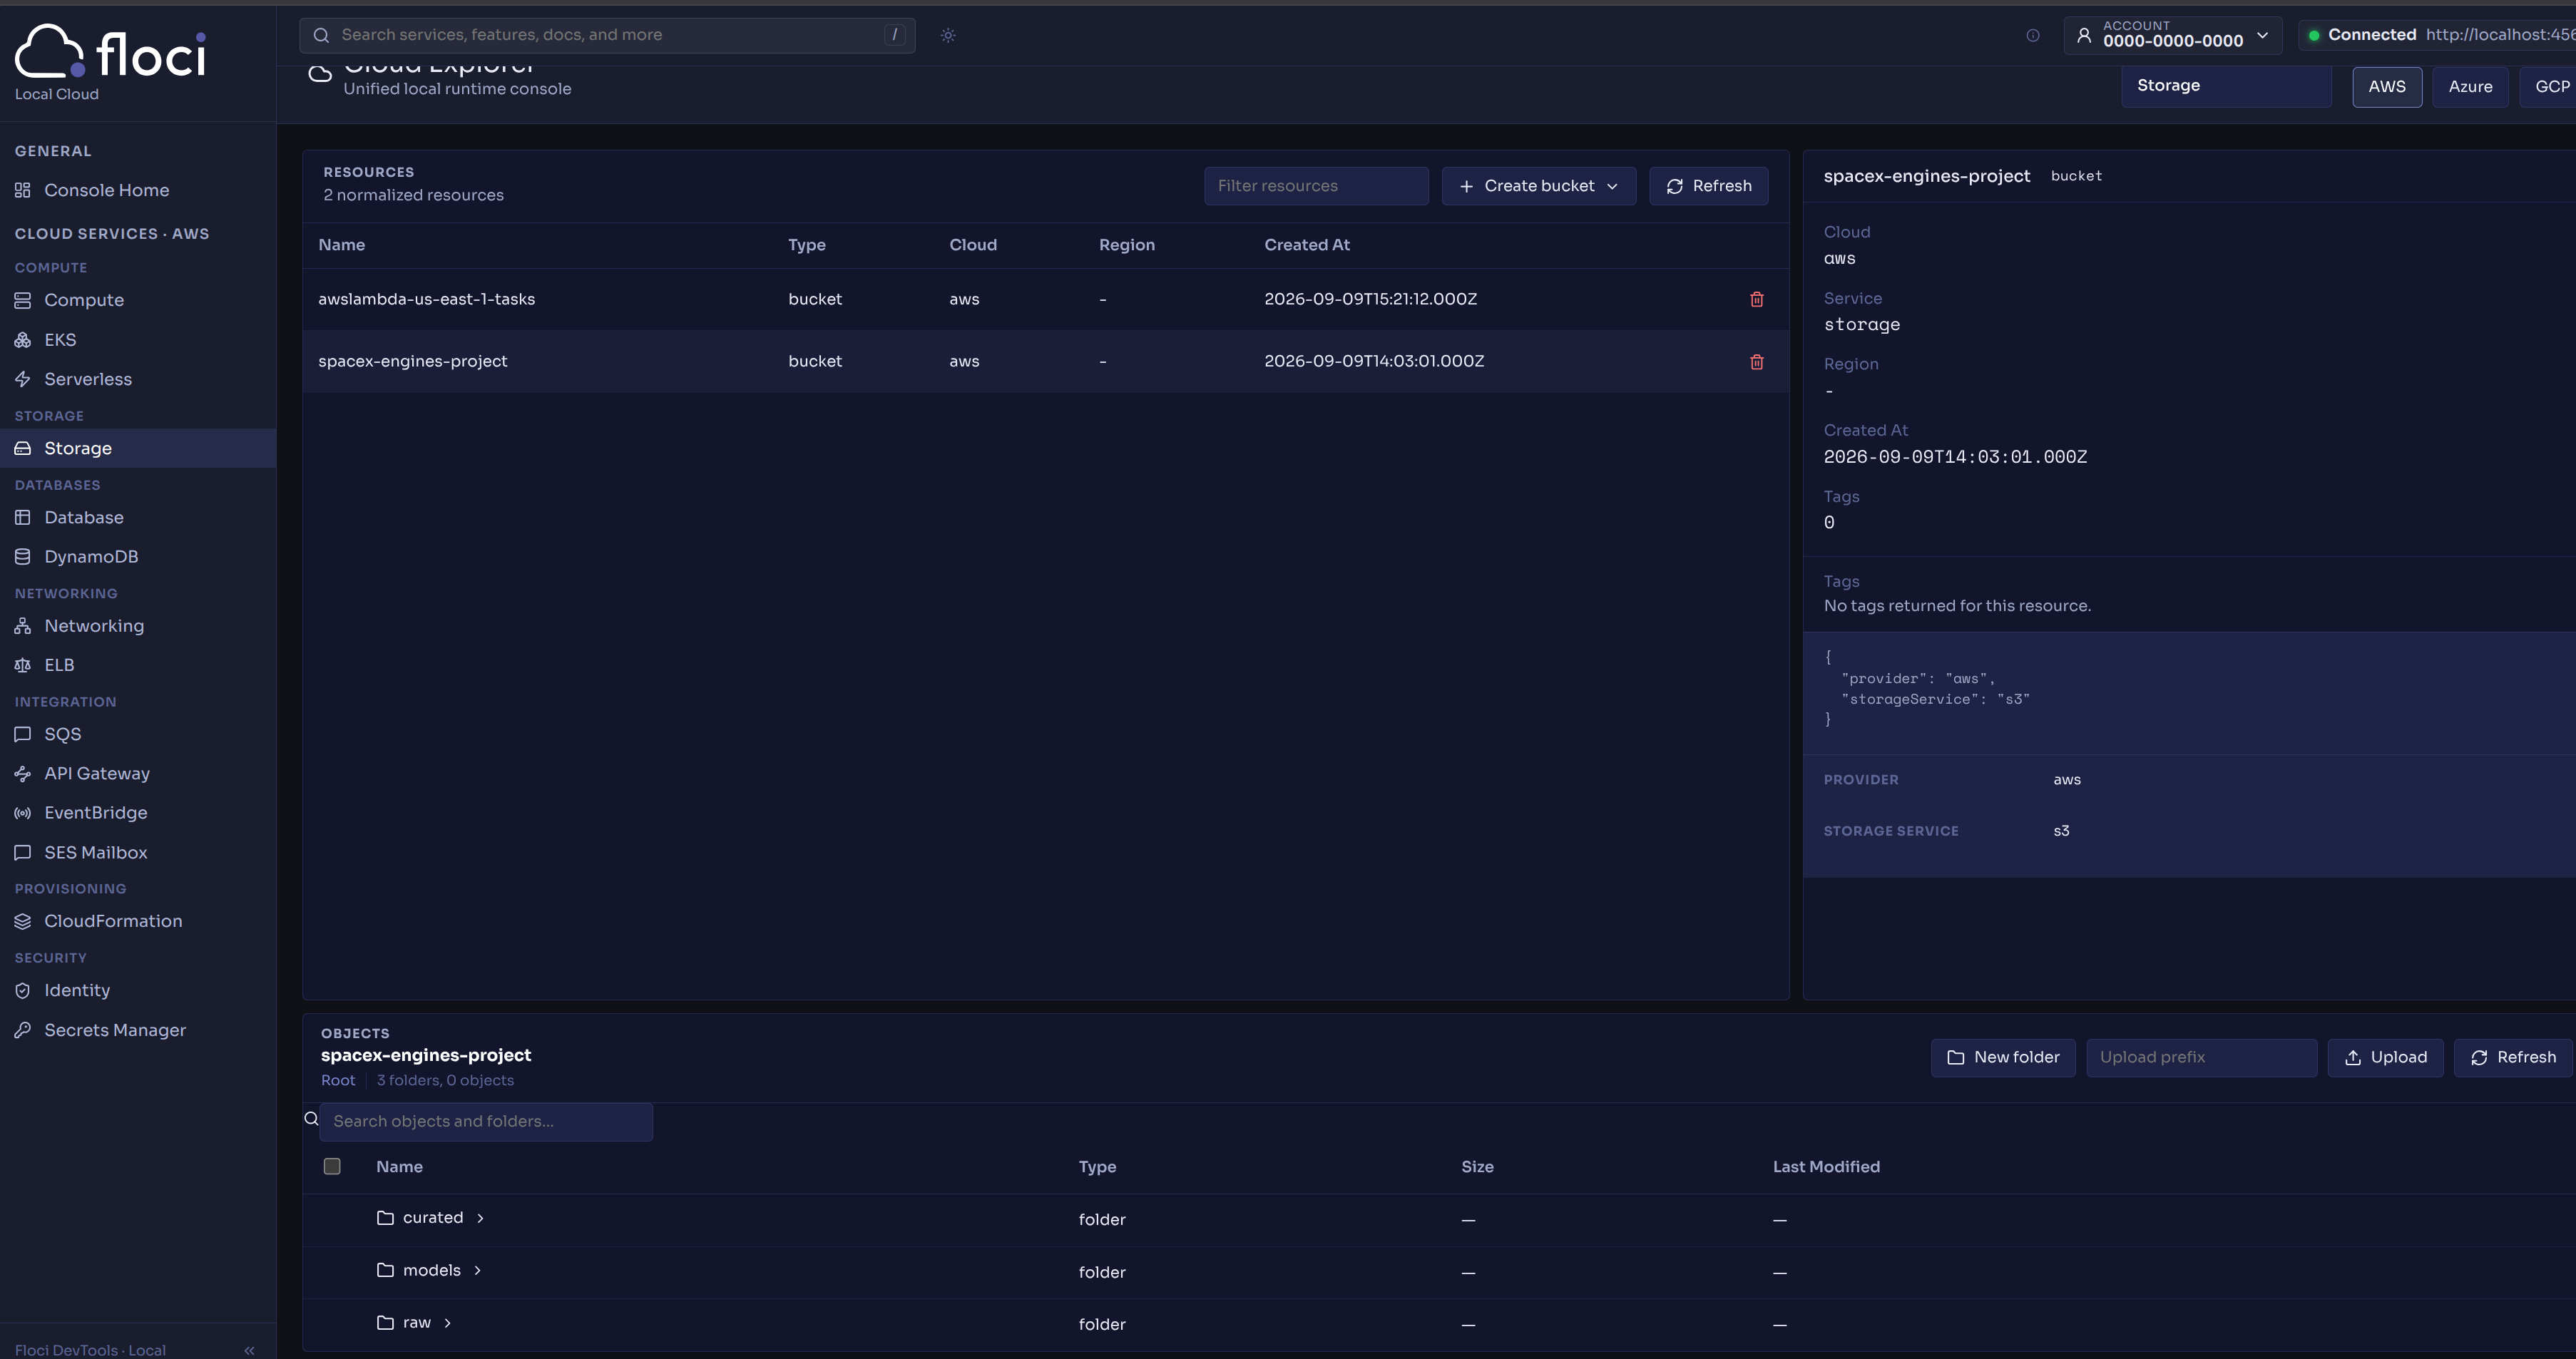
\includegraphics[width=0.85\textwidth]{flociS3.png}
    \caption{Bucket S3 local en Floci, con las carpetas \texttt{curated/}, \texttt{models/} y \texttt{raw/} ya pobladas.}
\end{figure}

\begin{figure}[h]
    \centering
    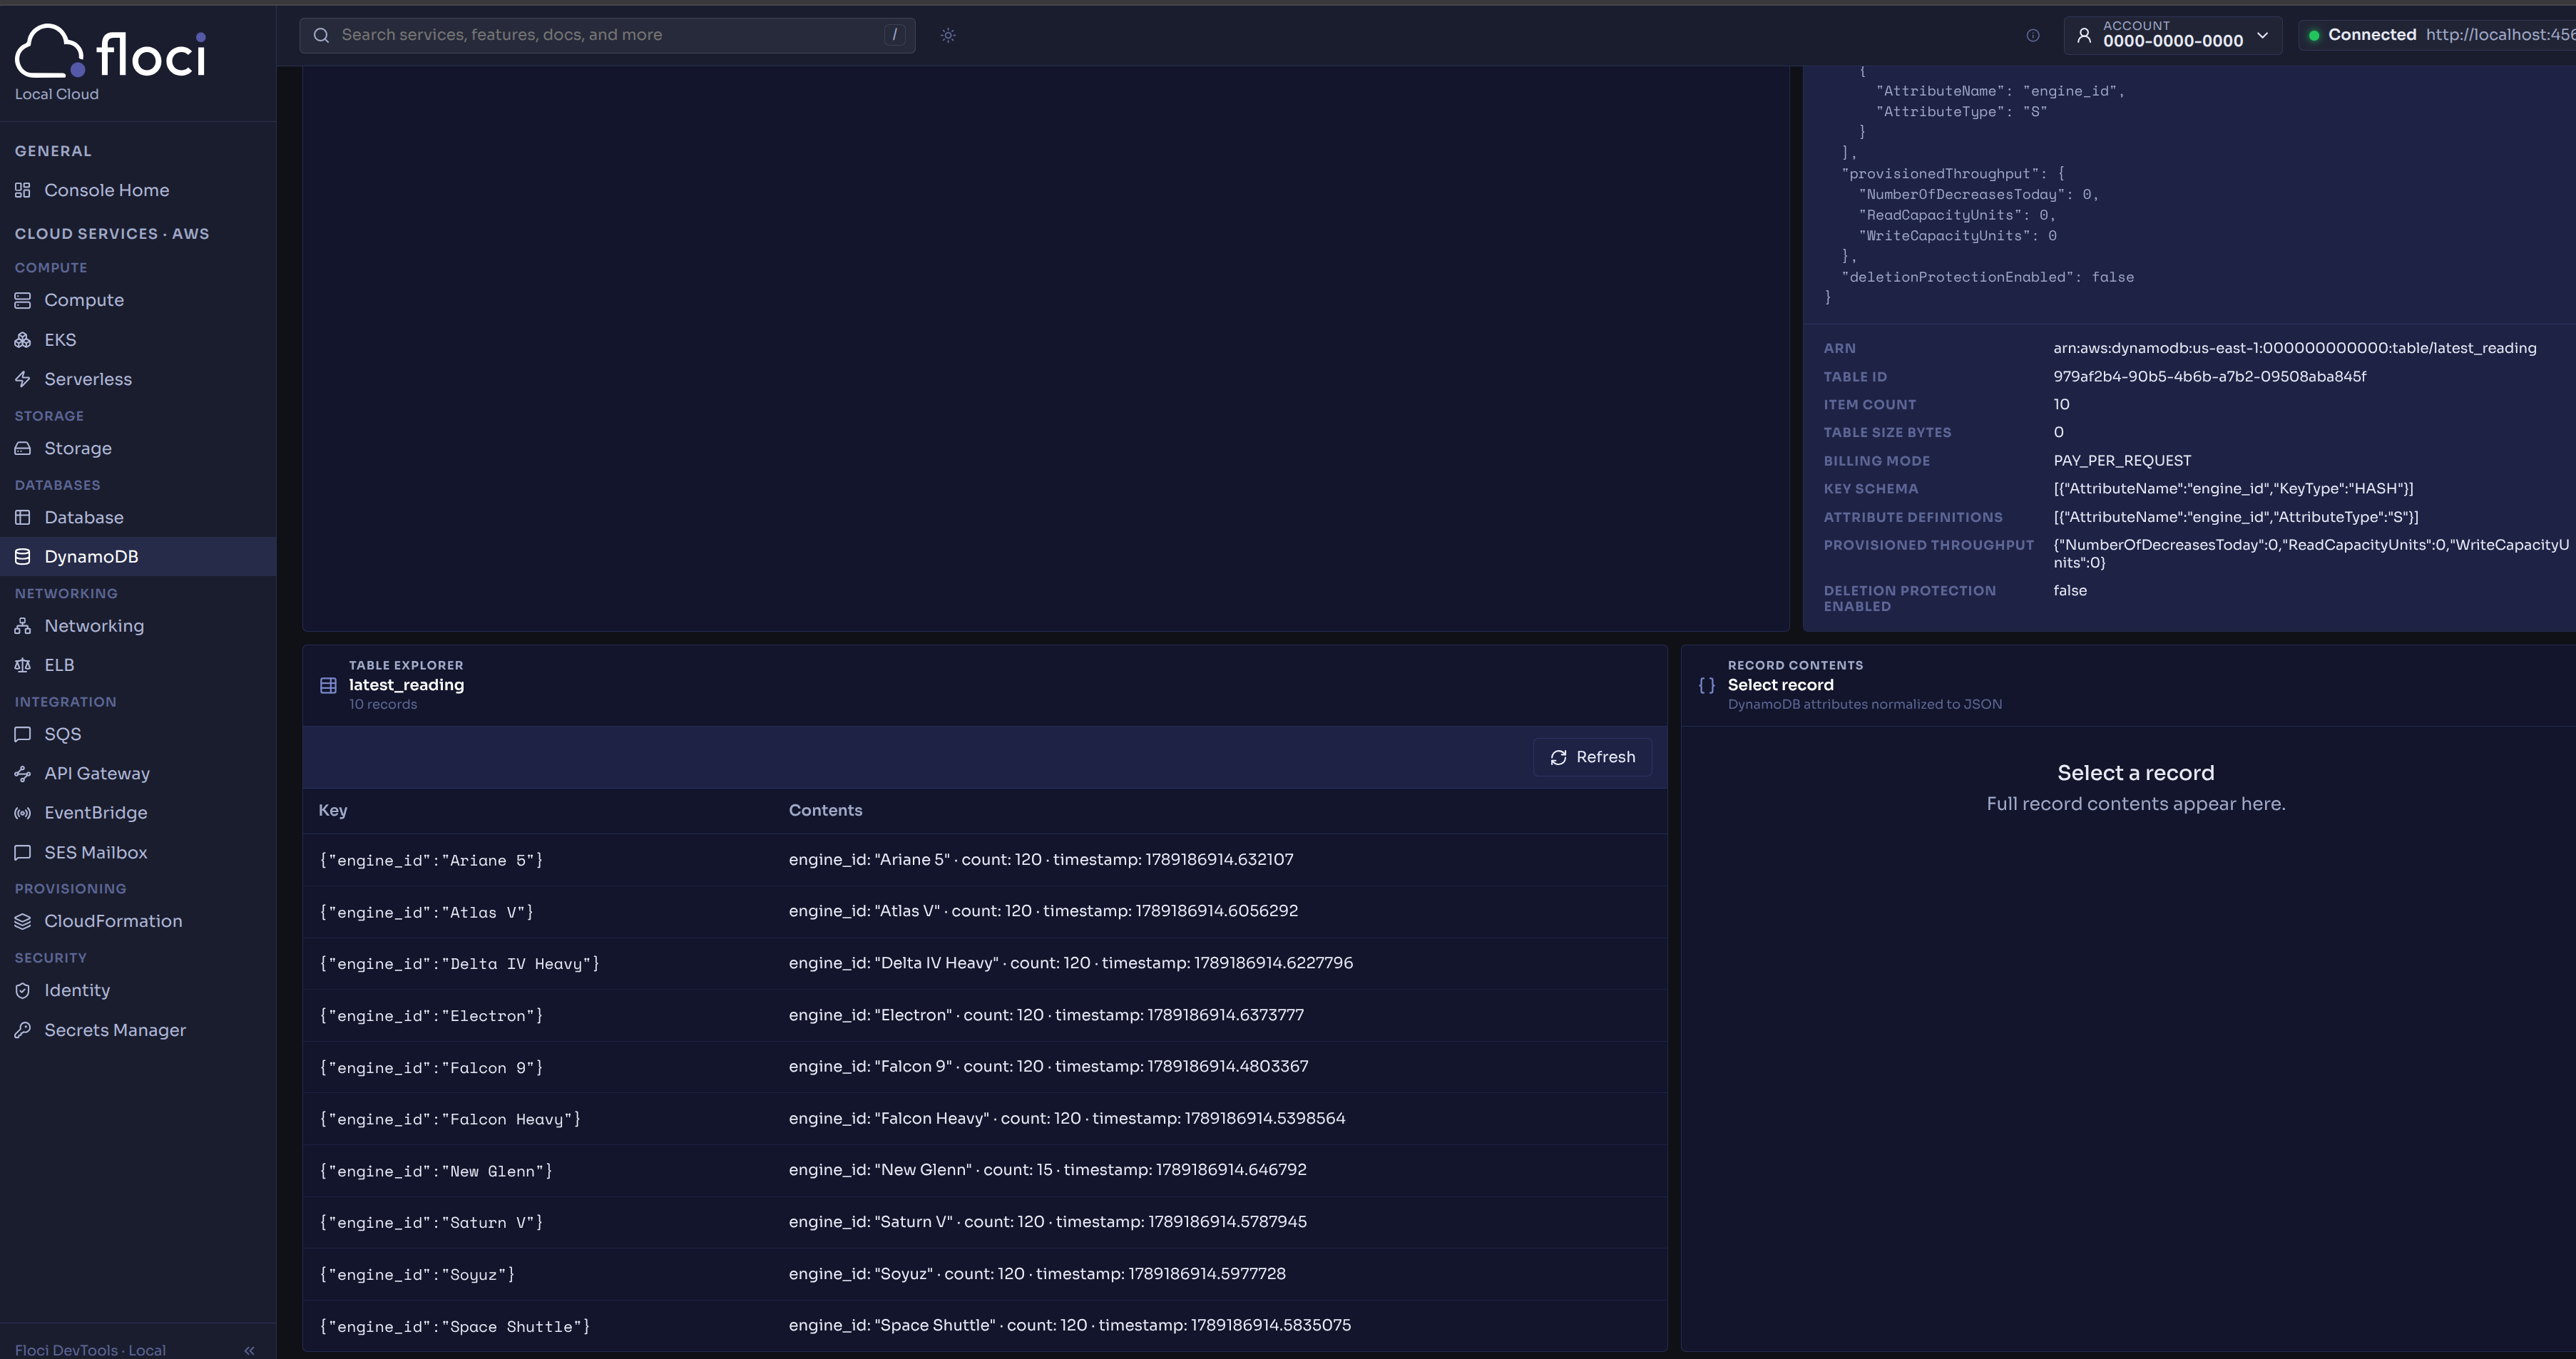
\includegraphics[width=0.85\textwidth]{flociDynamo.png}
    \caption{Tabla DynamoDB \texttt{latest\_reading} en Floci -- 10 registros, uno por motor (incluye New Glenn, agregado posteriormente).}
\end{figure}

\begin{figure}[h]
    \centering
    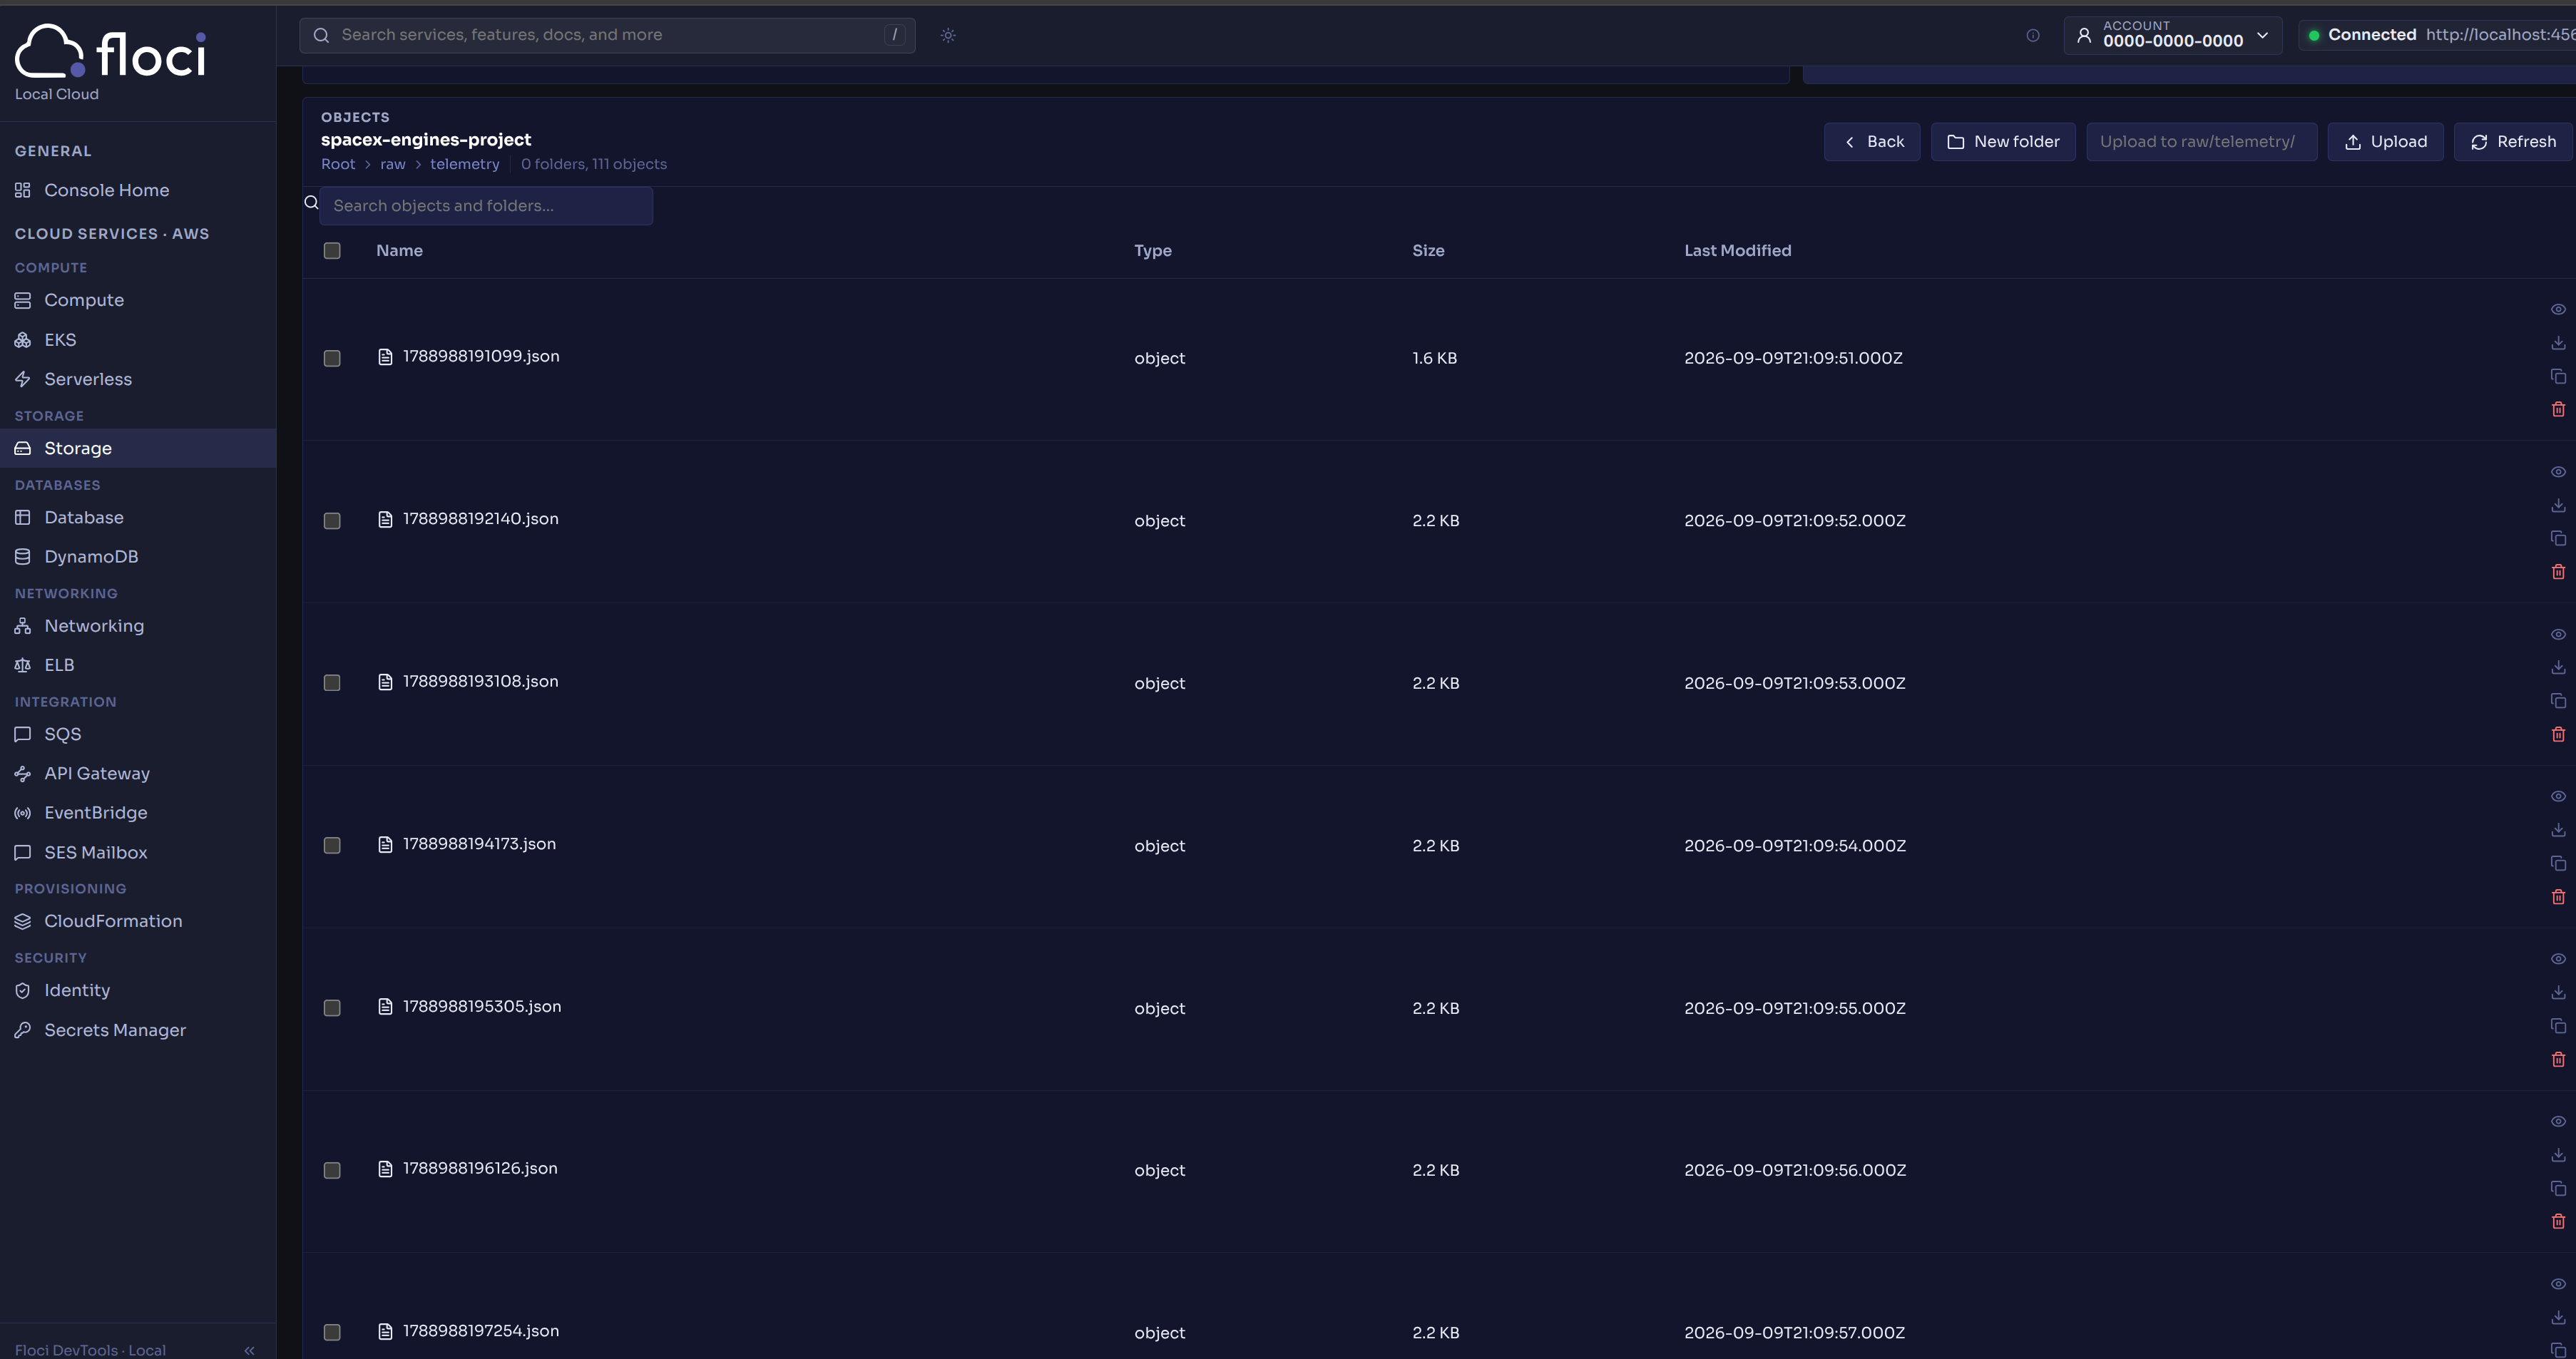
\includegraphics[width=0.85\textwidth]{flociS3telemetry.png}
    \caption{Histórico completo de lecturas de telemetría archivadas en S3 (\texttt{raw/telemetry/}) -- 111 objetos, cada uno correspondiente a una invocación de la Lambda consumidora.}
\end{figure}

\begin{figure}[h]
    \centering
    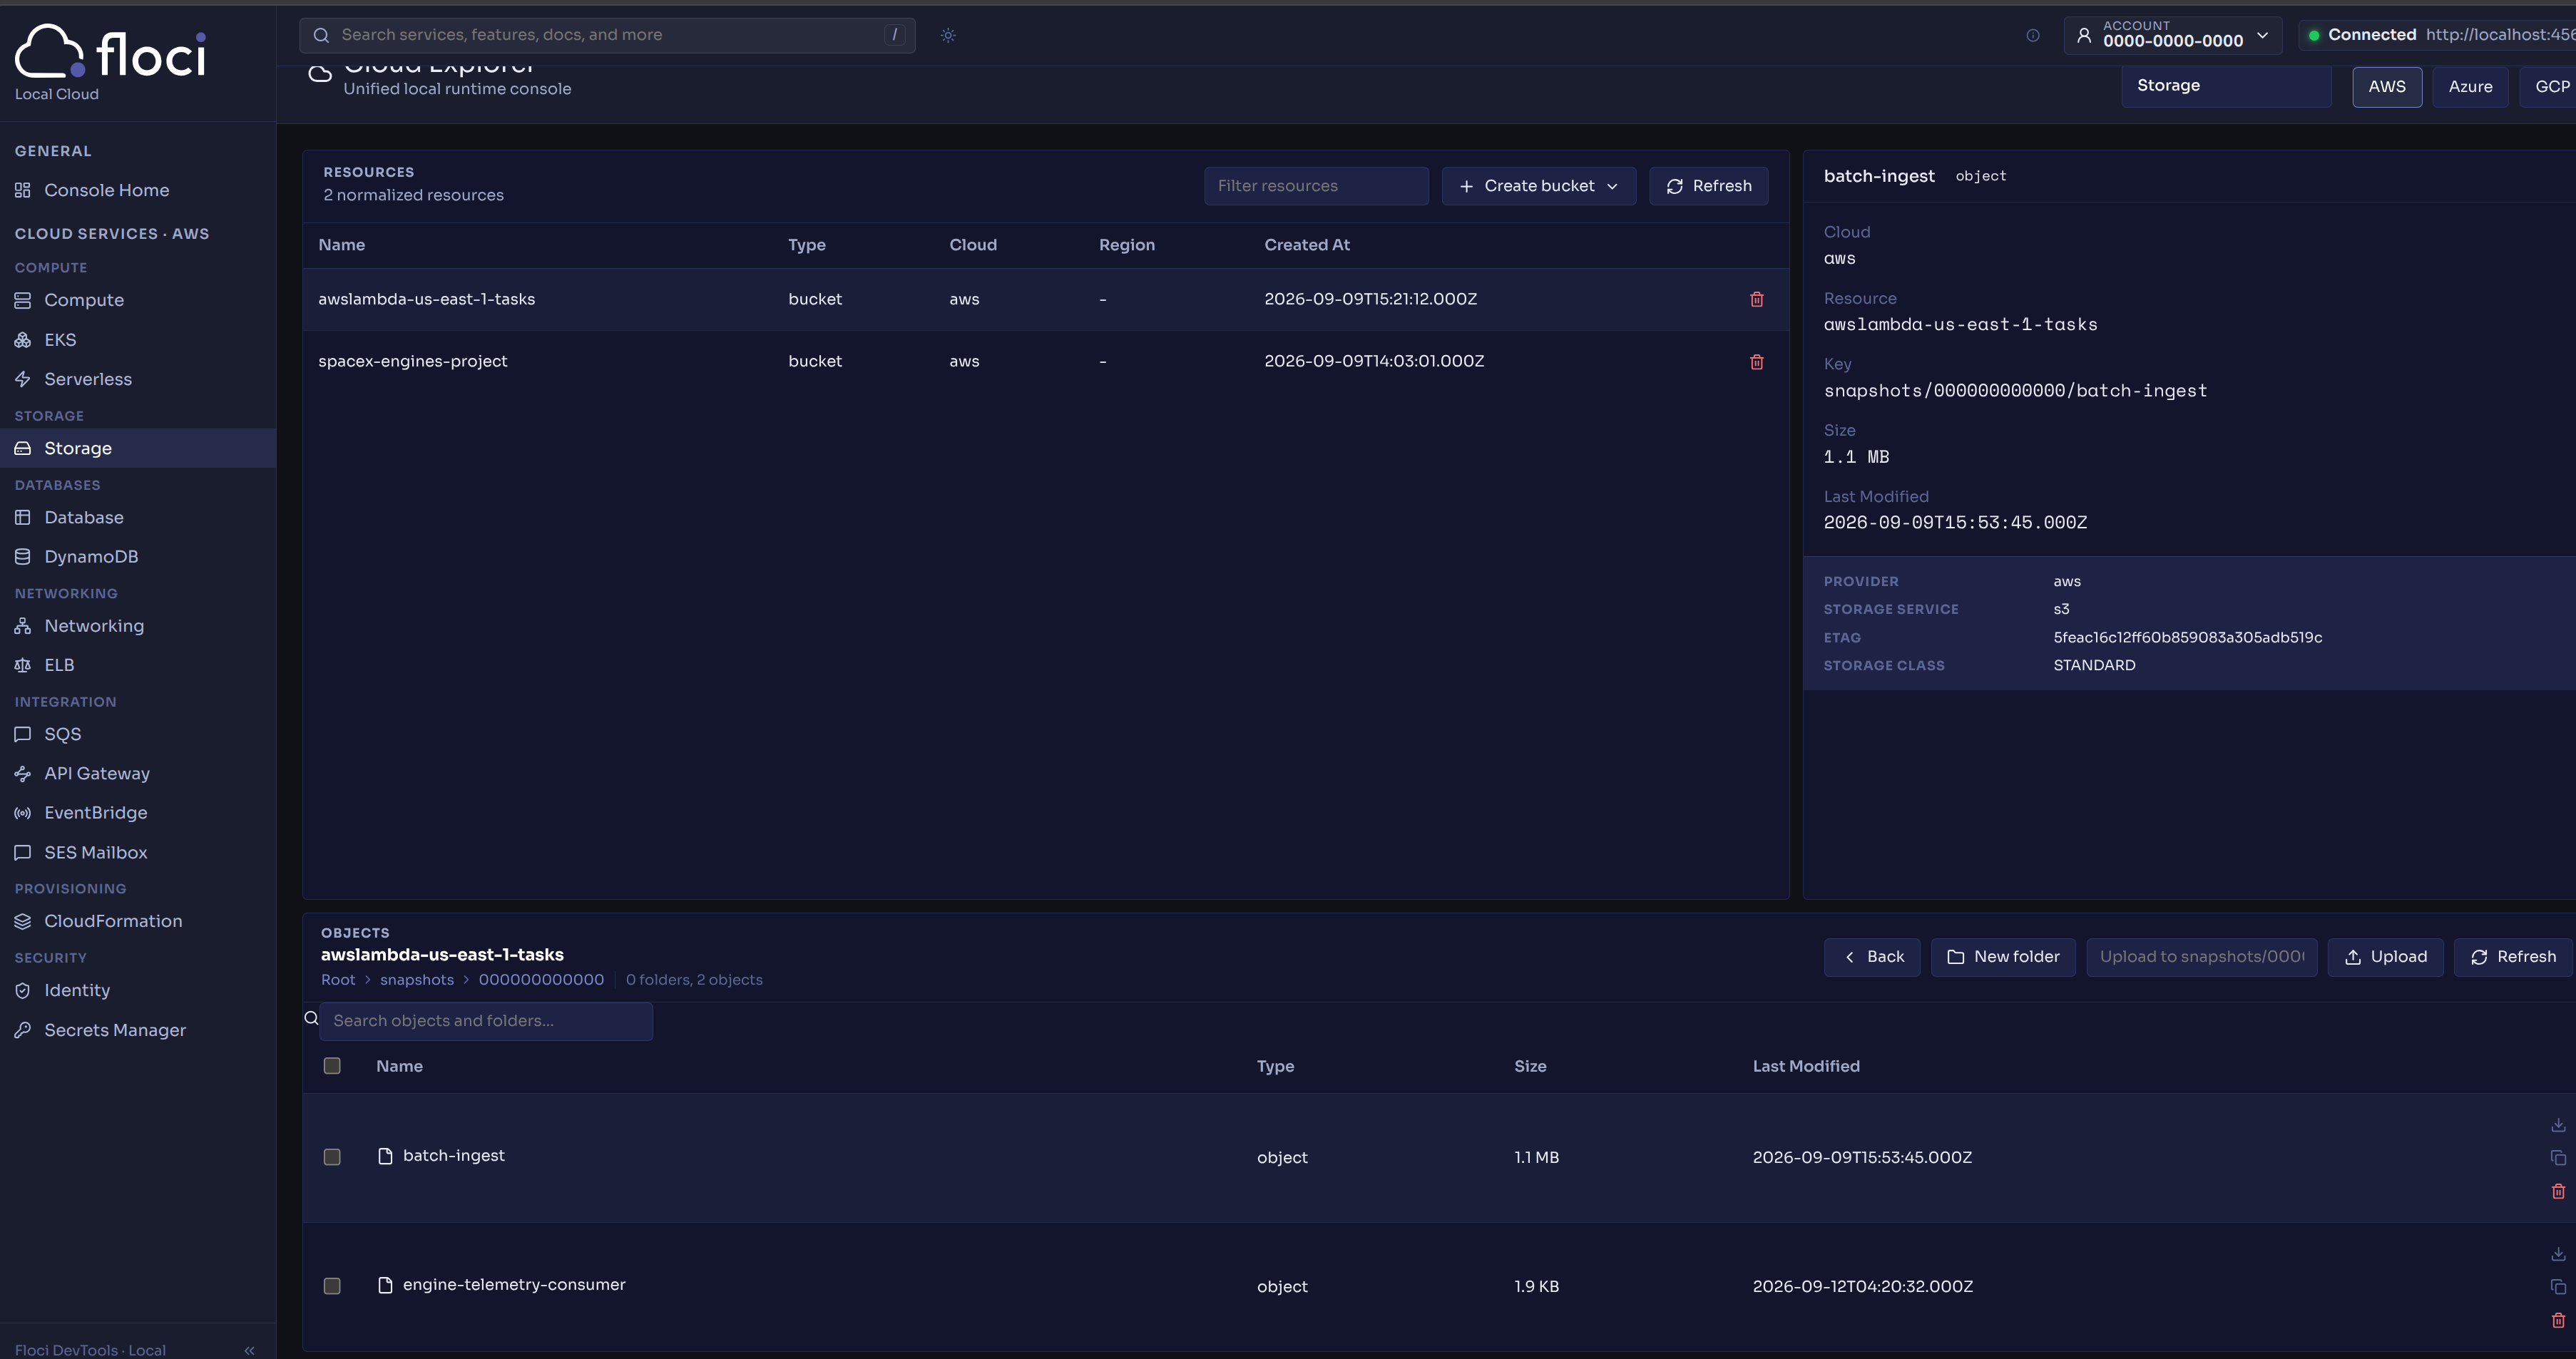
\includegraphics[width=0.85\textwidth]{flociS3lambdas.png}
    \caption{Paquetes de despliegue de las funciones Lambda (\texttt{batch-ingest}, \texttt{engine-telemetry-consumer}) almacenados internamente por Floci -- evidencia de que corren como funciones Lambda reales, no como scripts que simulan serlo.}
\end{figure}

\newpage
% ============================================================
\section{Despliegue en AWS real}
% ============================================================

Una vez validado localmente, el pipeline completo se desplegó contra una cuenta real de AWS, usando un usuario IAM dedicado y automatización vía GitHub Actions (ver Sección~\ref{sec:cicd}).

\begin{figure}[h]
    \centering
    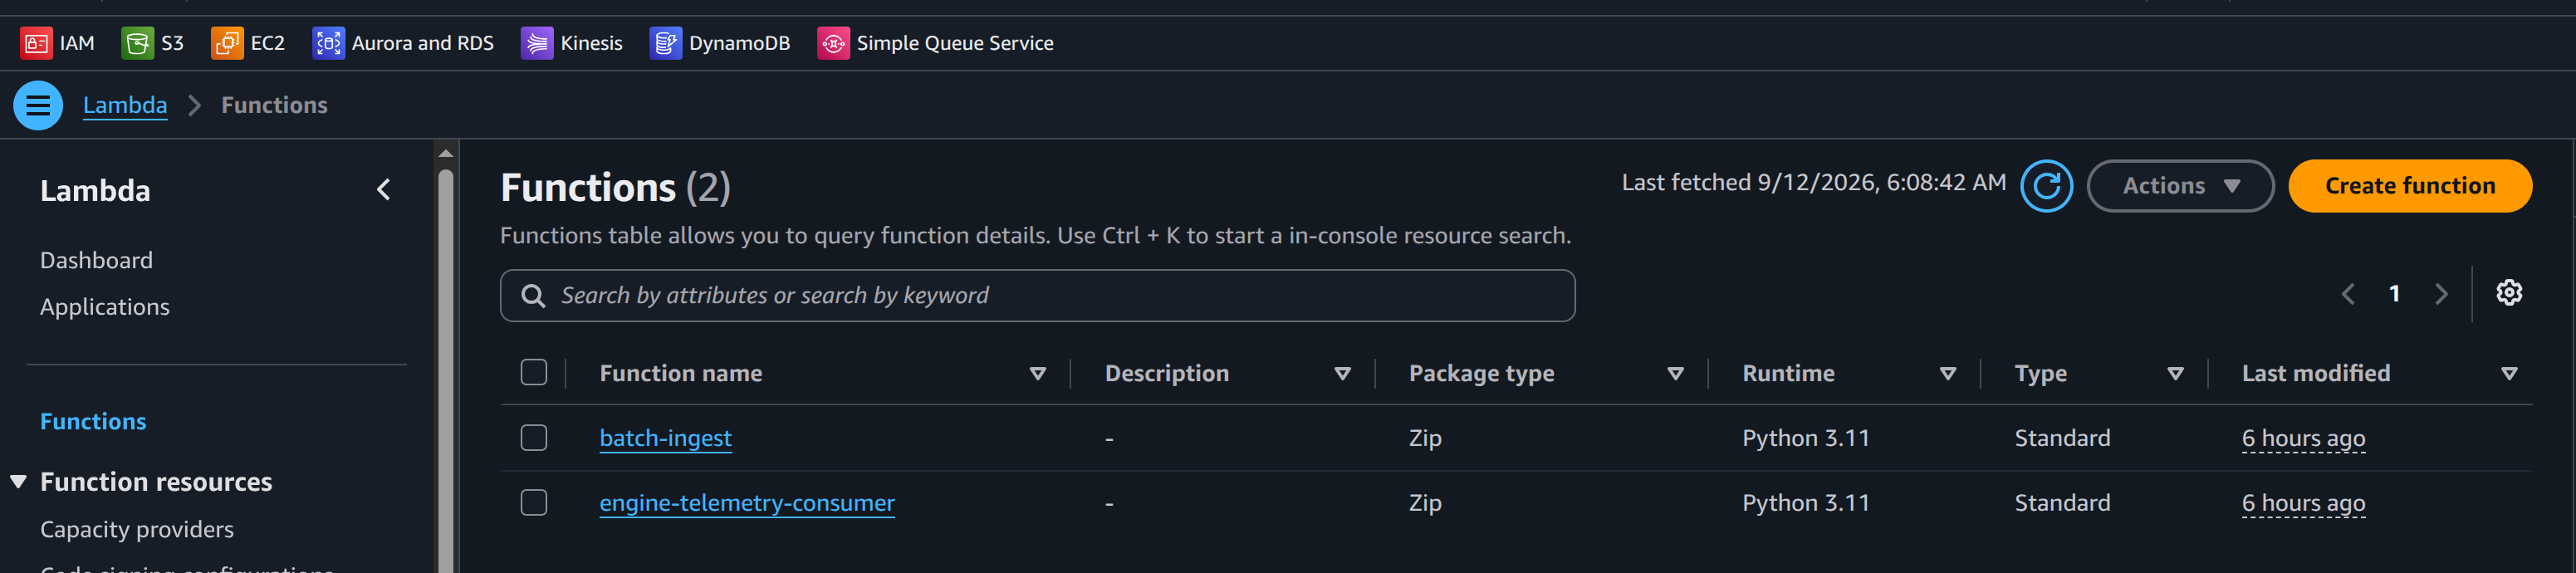
\includegraphics[width=0.85\textwidth]{lambdas.png}
    \caption{Las dos funciones Lambda reales desplegadas en la consola de AWS: \texttt{batch-ingest} y \texttt{engine-telemetry-consumer}.}
\end{figure}

\begin{figure}[h]
    \centering
    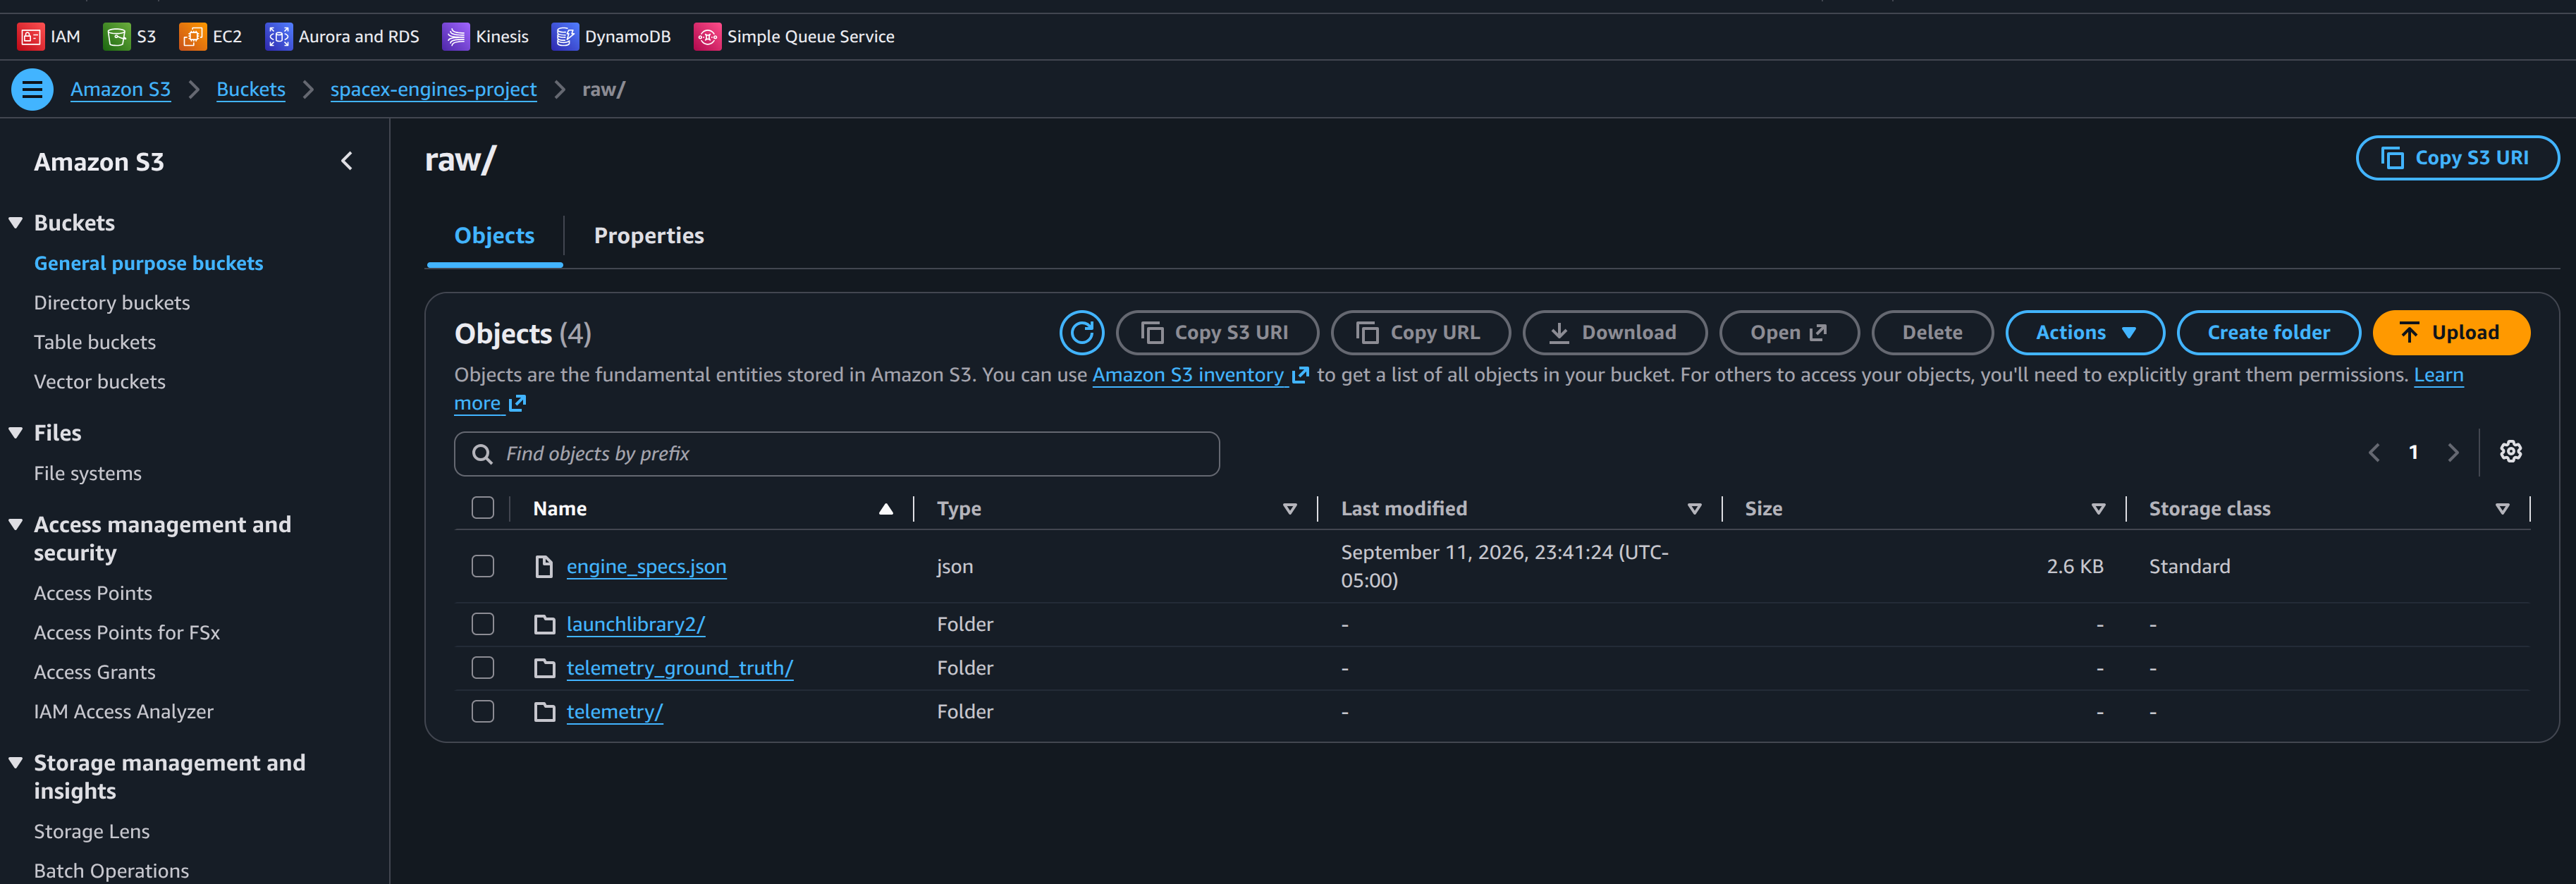
\includegraphics[width=0.85\textwidth]{AWS_S3.png}
    \caption{Bucket S3 real en AWS, con los datos crudos y curados del flujo batch.}
\end{figure}

\begin{figure}[h]
    \centering
    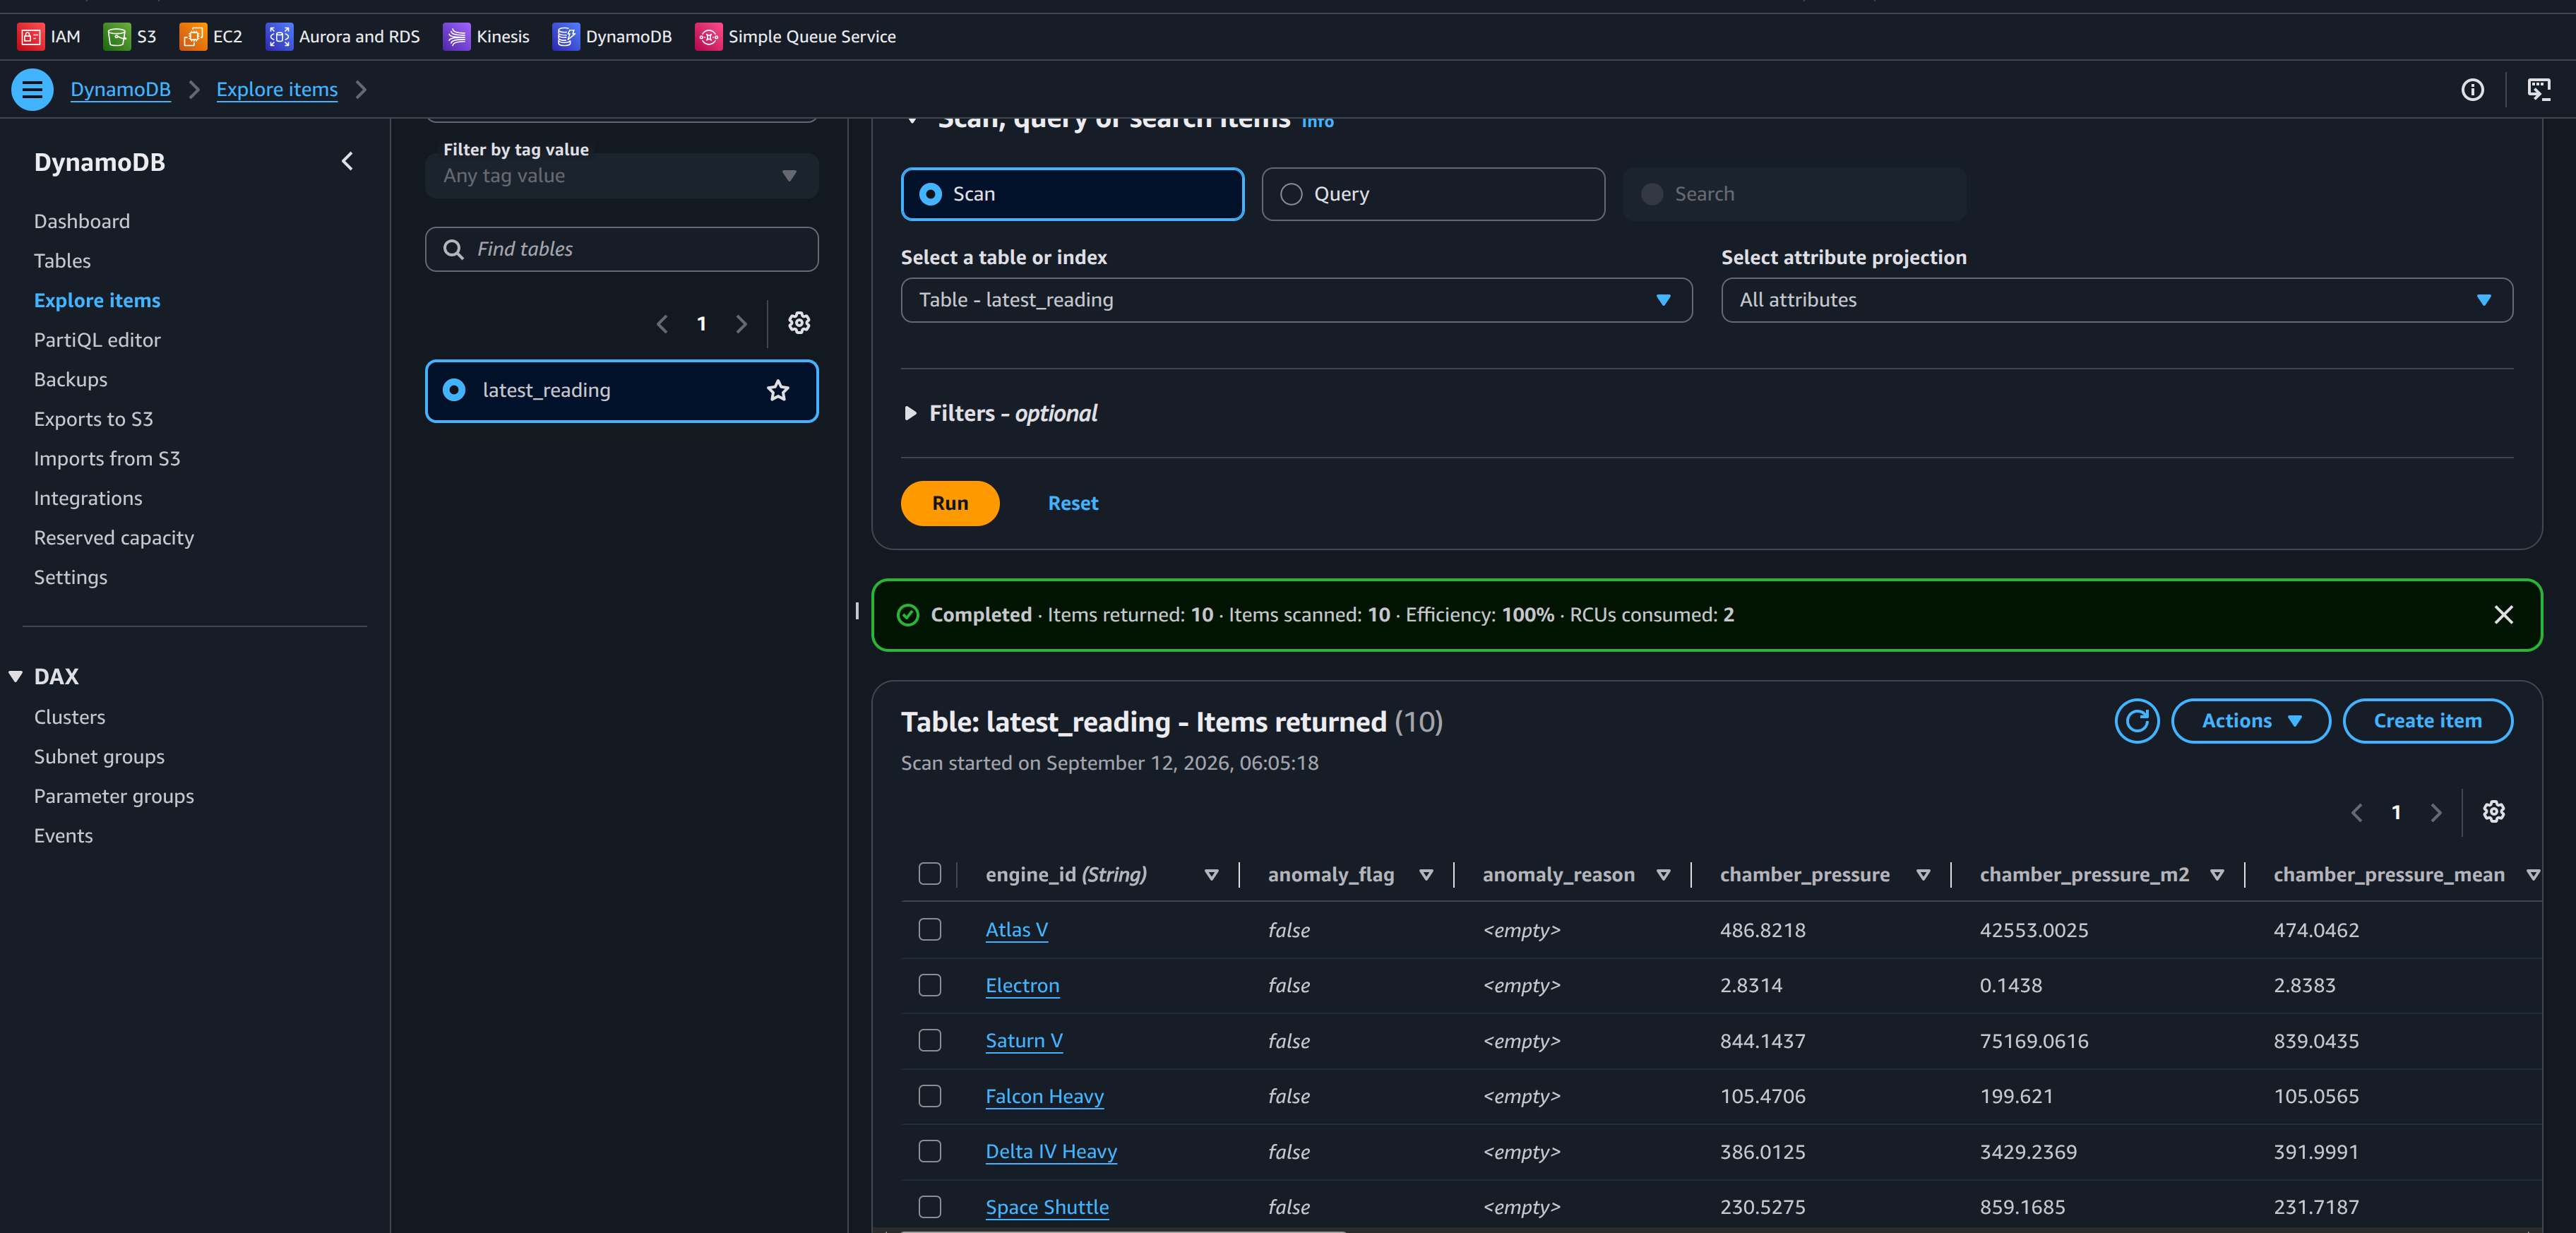
\includegraphics[width=0.85\textwidth]{DynamoAWS.png}
    \caption{Tabla DynamoDB \texttt{latest\_reading} en AWS real -- 10 elementos retornados, confirmando que el flujo streaming completo (SQS $\rightarrow$ Lambda $\rightarrow$ DynamoDB) funciona de punta a punta en producción.}
\end{figure}

\newpage
% ============================================================
\section{CI/CD -- Automatización con GitHub Actions}
\label{sec:cicd}
% ============================================================

El despliegue y la generación de datos de prueba contra AWS real están automatizados mediante dos \textit{workflows} de GitHub Actions, ambos de disparo manual (\texttt{workflow\_dispatch}):

\begin{itemize}
    \item \textbf{Deploy to real AWS} -- crea la infraestructura (bucket S3, tabla DynamoDB, cola SQS), despliega ambas funciones Lambda, ejecuta la ingesta batch, la transformación y el entrenamiento del modelo.
    \item \textbf{Run streaming producer (real AWS)} -- ejecuta el simulador de telemetría contra la cola SQS real, para poblar DynamoDB con datos en vivo bajo demanda (por ejemplo, justo antes de una demostración).
\end{itemize}

\begin{figure}[h]
    \centering
    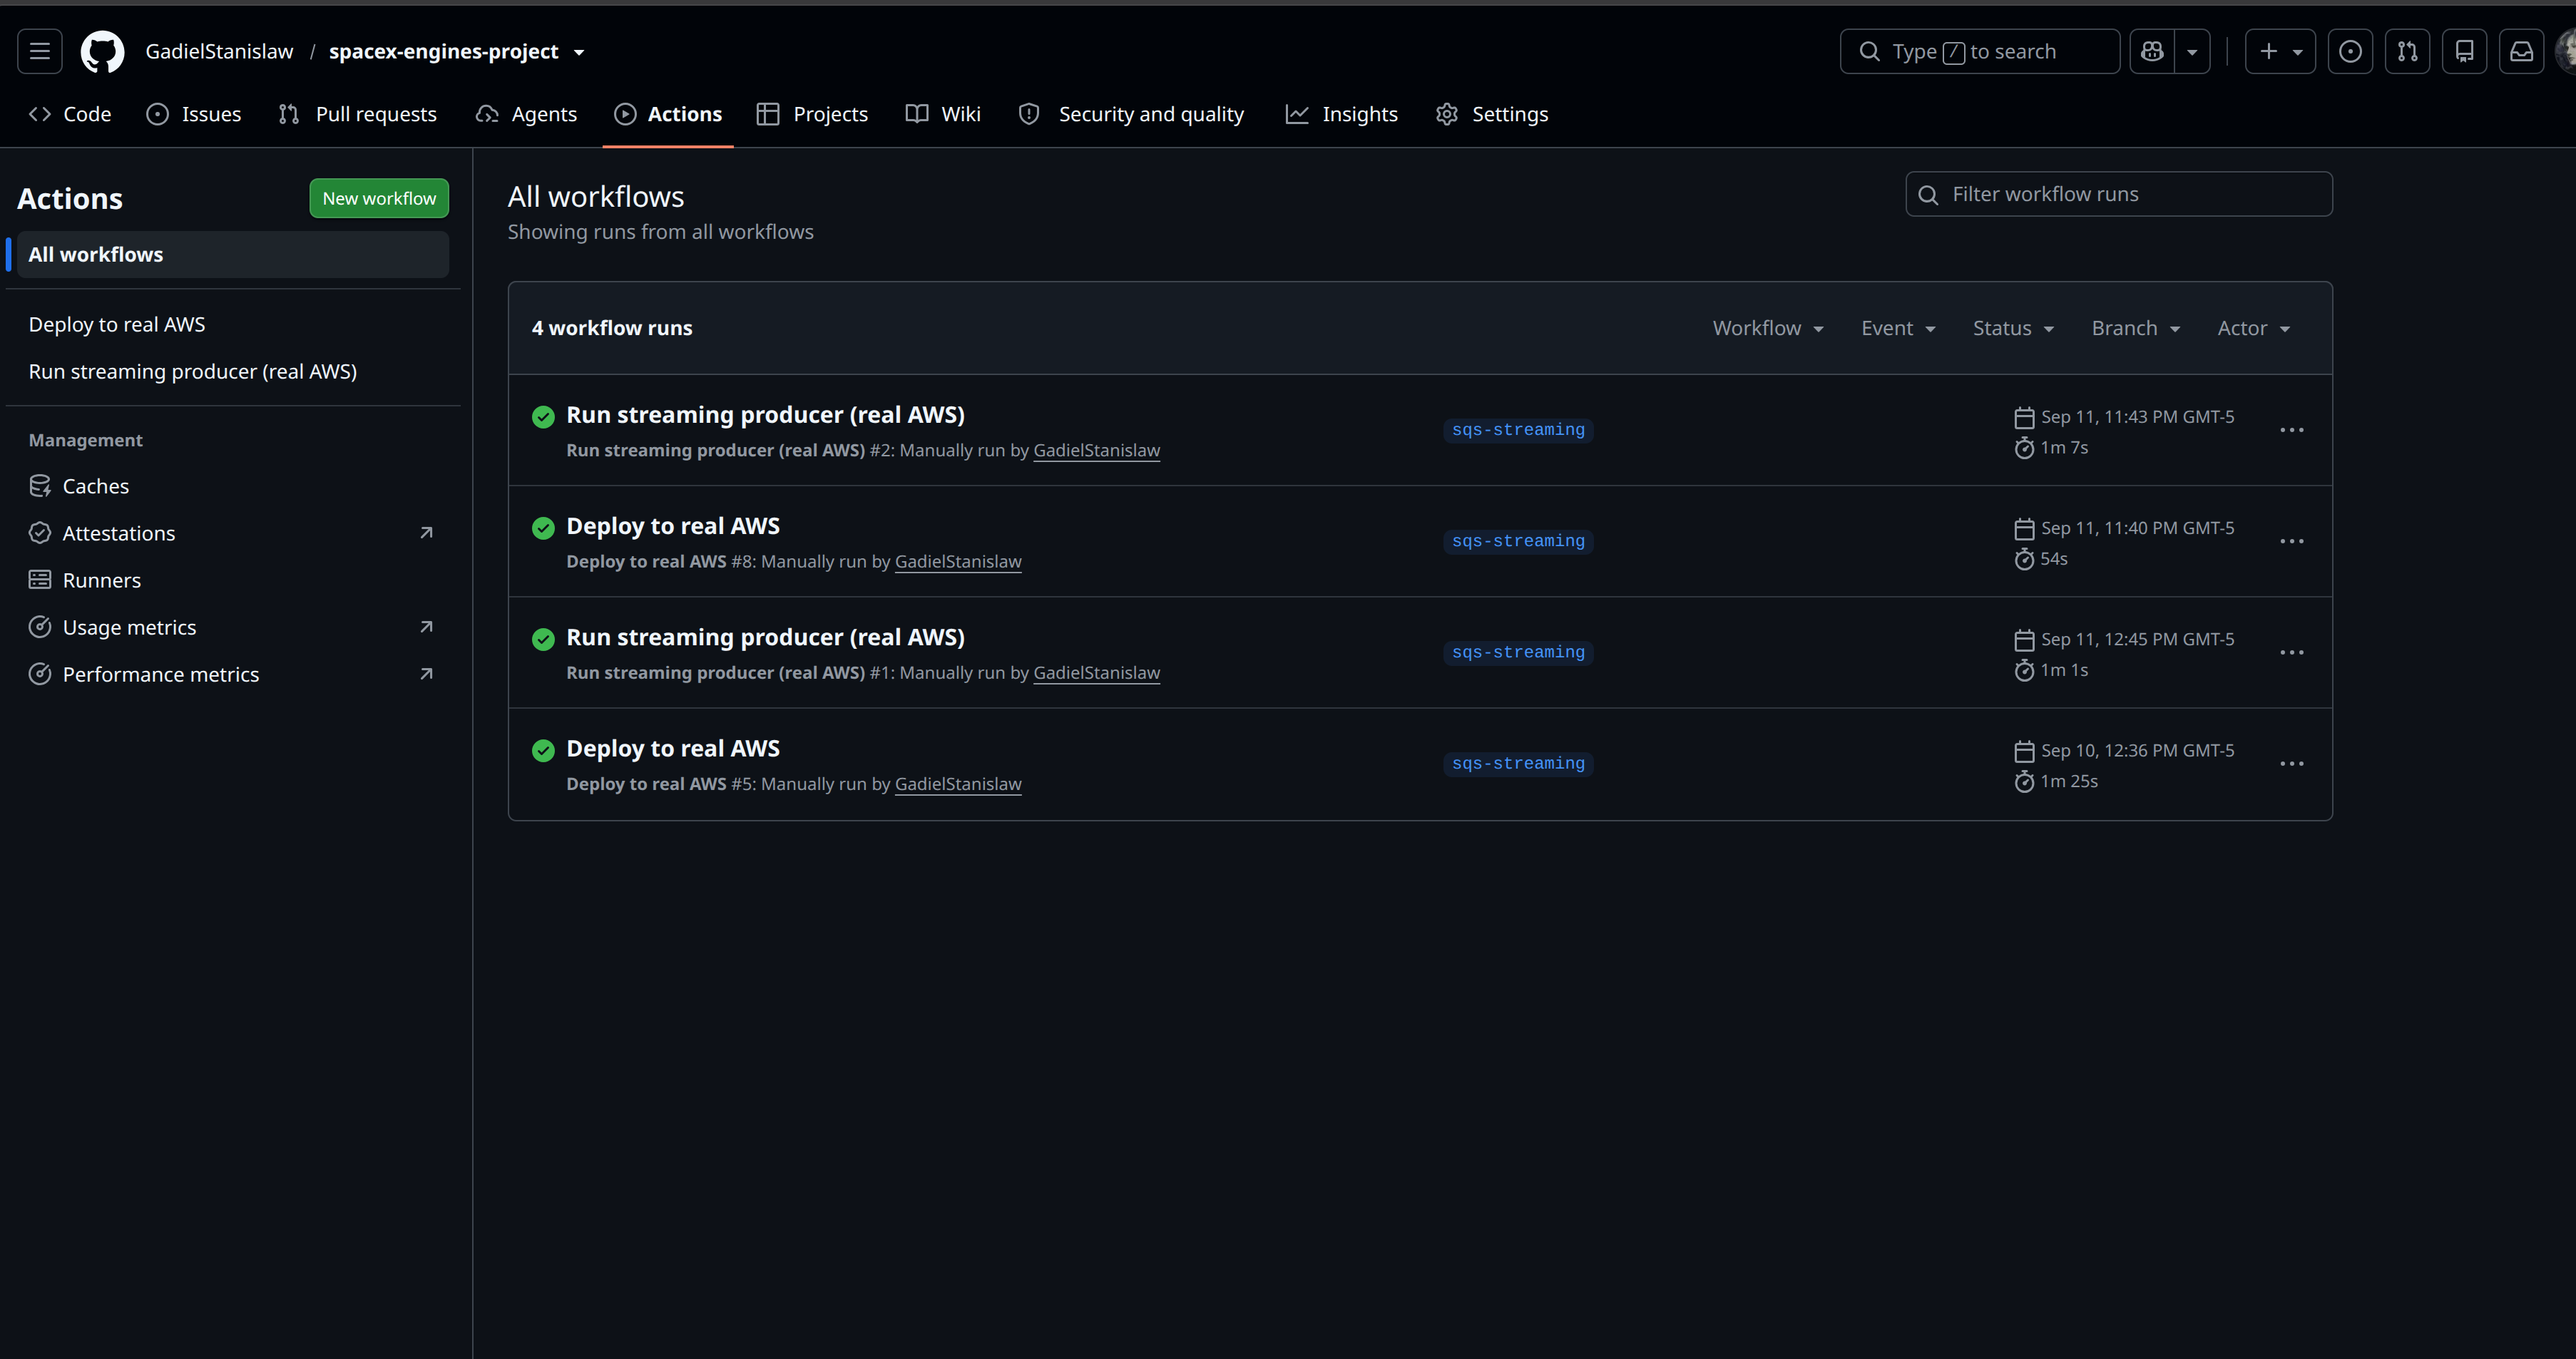
\includegraphics[width=\textwidth]{gihubrunners.png}
    \caption{Historial de ejecuciones exitosas de ambos workflows en GitHub Actions.}
\end{figure}

\newpage
% ============================================================
\section{Dashboard}
% ============================================================

\texttt{src/dashboard/app.py}, construido con \textbf{Streamlit}, consolida ambos flujos en una sola pantalla:
\begin{itemize}
    \item \textbf{Parte superior (batch):} métricas generales, gráfico de tasa de éxito por familia de cohete, e importancia de features del modelo -- incluyendo la limitación honesta del modelo predictivo.
    \item \textbf{Parte inferior (streaming):} tabla en vivo con el estado actual de cada motor, actualizándose automáticamente cada 3 segundos, resaltando en rojo los motores marcados como anómalos.
\end{itemize}

El mismo código del dashboard corre sin modificaciones contra Floci o contra AWS real.

% ============================================================
\section{Tecnologías utilizadas}
% ============================================================

\begin{table}[h]
\centering
\begin{tabular}{@{}ll@{}}
\toprule
\textbf{Categoría} & \textbf{Tecnología} \\
\midrule
Cómputo & AWS Lambda (2 funciones reales) \\
Mensajería & Amazon SQS \\
Base de datos & Amazon DynamoDB \\
Almacenamiento & Amazon S3 \\
Seguridad & AWS IAM \\
CI/CD & GitHub Actions \\
Entorno local & Floci (emulador AWS vía Docker) \\
Lenguaje & Python (boto3, pandas, scikit-learn, requests) \\
Formato de datos & JSON (crudo), Parquet (curado) \\
Visualización & Streamlit \\
Control de versiones & Git / GitHub \\
\bottomrule
\end{tabular}
\caption{Resumen de tecnologías por categoría.}
\end{table}

% ============================================================
\section{Conclusiones}
% ============================================================

El proyecto cumple con los requisitos del curso: ingesta desde múltiples fuentes, dos tipos de flujo (batch y streaming en tiempo real), procesamiento en tiempo real con detección de anomalías validada, almacenamiento en múltiples capas (cruda y curada), y despliegue real en la nube -- no simulado. El desarrollo local reproducible con Floci permitió iterar de forma rápida y sin costo antes de desplegar contra AWS real, y todo el código, tests y automatización de despliegue están versionados en el repositorio de GitHub del proyecto.

\end{document}
